% chap51.tex - 平台章子文件, 由 chap5.tex 通过 \input 引入
% 注: 本文件不带 \chapter{...}, 章节标题由父文件 chap5.tex 提供.
\section{引言}

强化学习在机器人控制中表现出较强的决策能力与环境适应性。
但在实际部署中，训练平台与真实机器人环境仍存在明显差异，且现有方法往往依赖高并行训练，而主流仿真平台（如 Gazebo、Webots）难以直接支持大规模并行。
因此，有必要构建兼具安全验证能力与工程可迁移性的中间验证平台，以缩小训练环境与真实系统之间的差距。

同时，安全验证过程需要在条件一致、流程可复现的实验设置下开展，以保证不同算法与控制模块在统一评价基准上的横向可比性，并减少由环境差异带来的评估偏差。

为构建安全基准，前两章已从不同层面提出多机器人安全强化学习方法，但这些方法主要在 \textit{Safety-Gymnasium} 中独立训练，尚未形成统一的工程执行链路。
在实际部署中，为同时兼顾安全性与任务性能，需要将强化学习策略、软协调机制与硬安全约束在统一系统中集成，并在标准化环境下开展系统验证，以提升方法的可复现性与可落地性。

基于上述需求，本文设计并实现了一套支持远程访问的面向多机器人安全强化学习的容器化仿真验证平台。
该平台基于开源教学系统 \textit{RoboticsAcademy} 进行扩展，通过引入面向多机器人编队任务的场景层、面向安全强化学习算法的容器化算法层，
以及面向分层控制的集成层与可复现评估管线，构建了完整的实验执行与评估体系。

在方法集成层面，本文将前两章提出的算法以
\[\text{MAPPO} \;\rightarrow\; \text{软协调层（GCPL）} \;\rightarrow\; \text{硬安全投影} \;\rightarrow\; \text{差速映射}\]
的串联形式进行统一整合。
其中，强化学习策略提供任务驱动的控制意图，软协调层在群体层面对多目标进行几何一致性优化，硬安全层对控制输入进行约束投影以保证严格安全性，最终通过差速映射生成可执行控制指令。
该分层控制结构在保持多目标协同能力的同时，实现了对安全约束的严格满足。

本文通过轻量级的 \textit{pure-python} MVP 系统对分层控制栈进行功能验证，并在 \textit{Webots} 高保真仿真环境中进行多场景实验评估。
实验结果表明，相较于单层控制方法，所提出的分层集成方案在安全性、任务完成度以及编队一致性等方面均取得了显著提升，从而验证了该平台及其控制机制的有效性与实用价值。

\section{平台总体设计}

% \subsection{对基础平台的功能需求}

% 为了实现多机器人安全强化学习方法的工程化验证与部署，平台不仅需要具备基础的机器人仿真能力，还必须在多智能体协同、安全约束执行以及实验可复现性等方面提供系统性的支持。
% 与传统单机器人仿真环境不同，多机器人场景对系统的建模能力、通信机制以及实验管理方式均提出了更高要求。

% 在任务执行层面，平台需要支持多机器人协同场景的构建与运行，即在同一仿真环境中实例化多个独立机器人个体（$N \ge 2$），并对其控制周期进行统一调度，从而为多智能体交互与编队任务提供基础支撑。
% 围绕算法运行需求，系统需提供完整的安全强化学习运行环境，包括深度学习框架 \textit{PyTorch}、 \textit{Safety-Gymnasium} 环境与 \textit{MAPPO} 等多智能体算法组件，
% 并支持对训练阶段生成的策略模型（checkpoint）进行加载与推理，从而实现训练与验证阶段的解耦。
% 在控制接口层面，平台需提供统一的多机器人状态访问与控制接口，包括位置、速度、朝向及邻居状态等信息的获取，以及多机器人控制指令的分发机制，以支持分层控制算法的集成与执行。
% 同时，平台应能够在统一代码路径下自动执行多算法、多随机种子的对比实验，并对实验结果进行集中整理与统计分析。通过构建标准化的实验流程，提升实验效率，同时保证结果的可复现性与可比性。
% 在可视化方面，平台不仅需要提供原生仿真界面的展示能力，用于场景调试与直观观察，还需支持结构化状态数据的可视化表达，以满足算法分析与性能评估需求。
% 为避免主机环境差异带来的影响，确保实验在不同设备与时间条件下的一致性，平台应采用容器化技术对运行环境进行封装，将所有依赖固化于镜像之中。

% 开源教学平台 \textit{RoboticsAcademy} 已在一定程度上满足了上述需求，例如其支持容器化部署、远程可视化（noVNC）以及机器人仿真环境（Gazebo）的集成。
% 然而，该平台主要面向单机器人教学任务，尚未支持多机器人调度机制、安全强化学习算法集成以及批量实验评估流程。
% 因此，本文的工作重点并非从零构建仿真系统，而是在其基础上进行针对性扩展，以满足多机器人安全强化学习的验证需求。

% \subsection{平台五层架构设计}

基于上述需求，本文对平台整体结构进行分层设计，将系统划分为自底向上的五个功能层次，如图~\ref{fig:platform_framework}所示。

最底层为仿真场景层，负责构建机器人运行的物理环境。该层以 \textit{Webots} 为核心工具，实现差速机器人建模、障碍物配置以及任务目标设置，为控制算法提供基础的动力学与感知支撑。
在此之上，控制接口层通过 \textit{ROS 2} 建立统一的通信机制。该层通过规范多机器人话题命名、状态采集与控制指令分发机制，实现机器人状态与控制信号的标准化交互，为分层控制算法提供统一的数据接口。
算法容器层对强化学习算法运行环境进行封装。借助 Docker 容器，深度学习框架与安全强化学习相关依赖被统一集成，同时支持策略模型的加载与执行，从而保证训练环境与验证环境的一致性。
分层集成层，用于实现第三章硬安全机制与第四章软协调机制的统一融合。通过将强化学习策略输出、几何协调过程以及安全约束投影按序串联，形成完整的控制管线，使系统在满足安全约束的同时具备良好的协同控制能力。
最上层为评估管线层，负责实验流程管理与结果分析。该层支持批量实验调度、消融实验配置以及自动化结果统计与可视化，从而实现对不同算法性能的系统性比较。

相较于原始 \textit{RoboticsAcademy} 平台，本文在多个层面进行了扩展与改造。仿真场景由单机器人任务扩展为多机器人编队环境，同时控制接口从单体 API 演化为多智能体通信体系。
算法运行环境引入安全强化学习相关依赖，并分层控制结构实现了软约束与硬约束的统一集成。此外，实验评估流程由单次运行扩展为支持批量对比与自动分析的完整管线。
通过上述设计，平台实现了从仿真环境构建、算法执行到实验评估的完整闭环，为多机器人安全强化学习方法的验证与工程应用提供了统一且可扩展的基础支撑。
\begin{figure}[htbp]
    \centering
    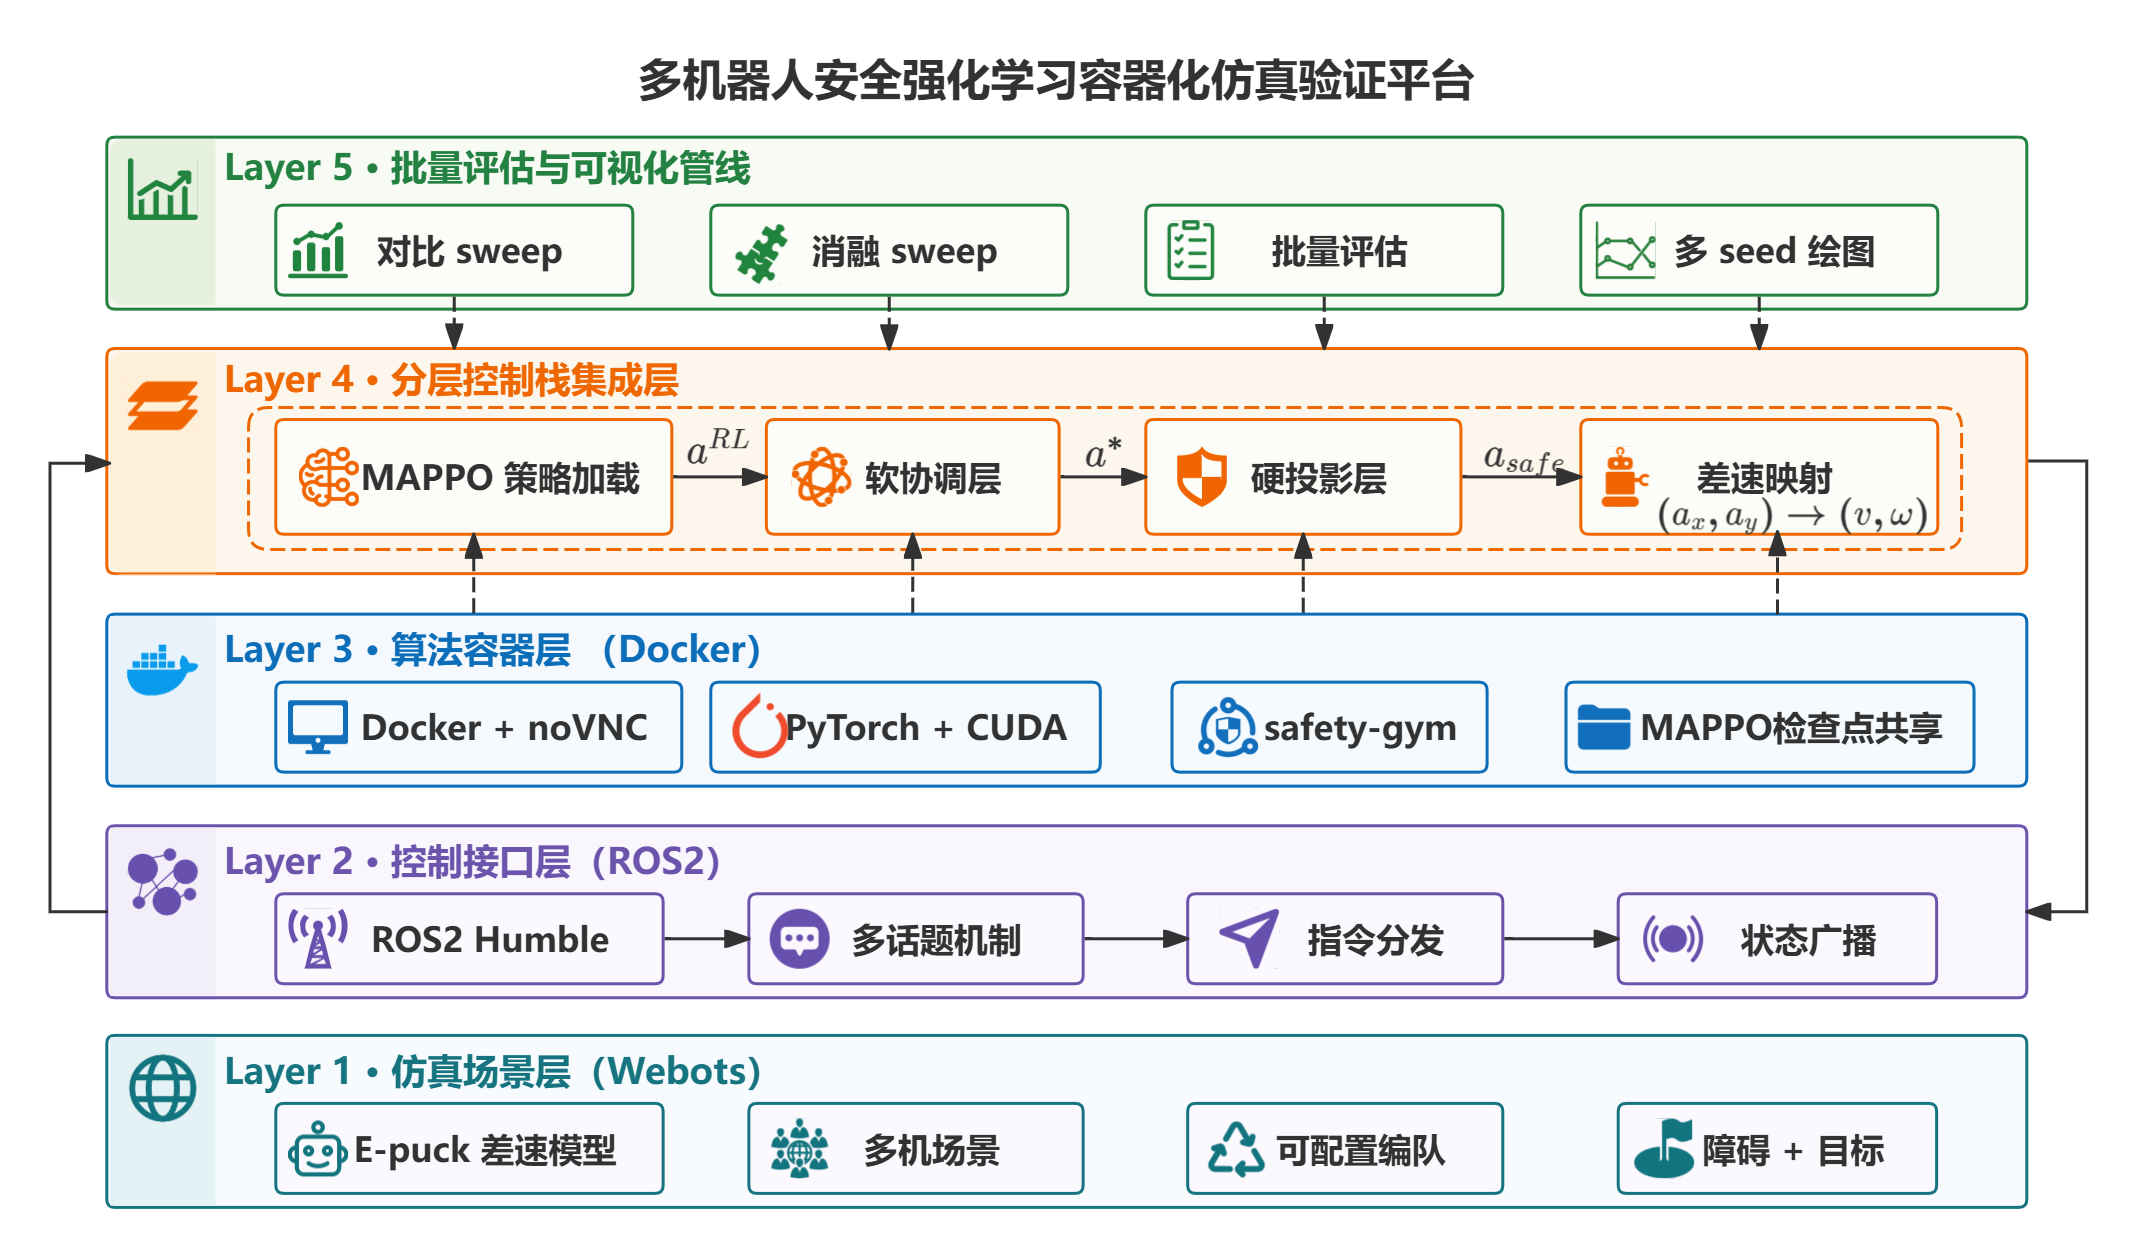
\includegraphics[width=\linewidth]{images/chap5_architecture.png}
    \caption{多机器人安全强化学习容器化仿真验证平台的五层架构}
    \label{fig:platform_framework}
\end{figure}

\section{核心机制与关键改进}

% 在上述分层架构基础上，为提升平台在安全强化学习场景下的易用性，本文围绕实验可复现性、系统可解释性以及交互实时性，设计了三项关键机制：
% 容器化并行调度机制、双通道可视化机制以及基于 WebSocket 的实时通信机制，从而提升平台性能与用户体验。

\subsection{容器化与并行调度机制}

针对强化学习算法对高并行训练环境的需求，以及机器人仿真环境在部署与依赖管理方面的复杂性，平台采用基于 Docker 的容器化运行机制对实验环境进行统一封装。

容器化运行机制中，每个实验任务均运行于独立的容器实例中，容器内部集成仿真引擎（如 Gazebo、Webots）、ROS 2 中间件以及算法执行模块。
该设计使不同实验之间在软件依赖、运行状态及资源使用上实现完全隔离，从而避免环境冲突问题。
同时，容器镜像在构建阶段已固定所有依赖版本，确保实验在不同时间与不同设备上的一致性，从而提升实验结果的可复现性。

在原有平台镜像基础上，本平台进一步集成深度学习框架与安全强化学习相关组件，从而构建完整的算法运行环境。
通过在容器内引入 PyTorch 及其相关依赖，并挂载外部代码目录的方式，将 Safety-Gymnasium 环境与 safepo 算法库以可编辑形式集成至容器中，使算法模块能够直接调用对应接口，以支持策略网络的加载与推理。
同时，前述安全算法相关实现作为独立模块进行管理，并通过环境变量实现路径配置，从而保证系统结构的清晰性。

在此基础上，平台通过容器调度机制支持多实例并行运行。后端系统根据用户请求动态创建、启动或销毁容器，实现实验任务的按需分配与资源管理。
该机制不仅能够支持多用户并发访问，还可为强化学习算法提供并行环境，从而提升样本采集效率与训练速度。
容器化与并行调度的完整数据链路如图~\ref{fig:chap5_parallel_orch} 所示：统一镜像经 build 阶段固定全部依赖后由调度器按需派生 $K$ 个隔离容器实例，
各容器内部独立运行 Webots 仿真、ROS\,2 桥接与 MAPPO + 安全栈，rollout 数据经共享卷汇聚至 MAPPO 训练器进行参数更新，更新后的策略再经同一卷下发至各容器，
形成并行采样、集中训练、异步推送的闭环。

\begin{figure}[htbp]
    \centering
    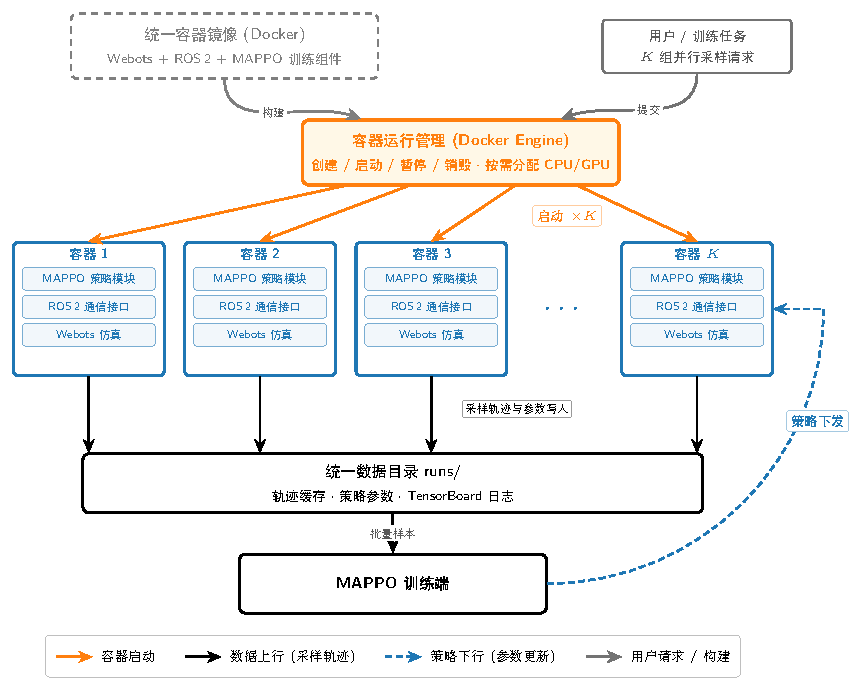
\includegraphics[width=0.95\linewidth]{figs/chap5_parallel_orchestration.pdf}
    \caption{容器化与并行调度机制}
    \label{fig:chap5_parallel_orch}
\end{figure}

\subsection{双通道可视化机制}

为提升机器人系统运行状态的可解释性与调试效率，平台设计了一种融合语义级状态表达与原生仿真界面展示的双通道可视化机制。
该可视化机制通过语义层表达与原生图形复现的协同设计，同时支持对算法状态的细粒度分析与对仿真场景的完整观测，从不同维度增强系统整体的可视化表达能力。

双通道并行的整体数据链路如图~\ref{fig:chap5_dual_vis} 所示。
语义级可视化通道（WebGUI）从仿真环境中提取机器人位姿、传感器读数以及安全约束等关键状态信息，并将其统一组织为结构化数据，通过 WebSocket 实时推送至前端。
前端采用组件化渲染方式，将上述数据映射为轨迹曲线、激光扫描、力向量以及约束边界等二维或抽象图形，从而直观呈现算法的内部状态与决策过程，使系统运行逻辑具备更强的可分析性与可解释性。

原生界面可视化通道（noVNC）则对仿真软件（如 Gazebo、RViz 或 Webots）的图形界面进行远程转发。
同源的仿真器图形界面在 Xvfb 承载下由 Xvnc 编码为 VNC 帧流，经 noVNC 客户端解码后以 iframe 嵌入前端页面，从而完整保留原生仿真工具的交互能力与视觉效果，使用户能够获得与本地运行一致的使用体验。

两条通路互不阻塞，前端用户交互指令经反向控制链路下发至仿真器，完成可视化与控制的闭环。图~\ref{fig:chap5_dual_vis} 的主要作用是显式刻画两条通路的"共源异构"关系与解耦运行边界：
一方面通过共享仿真器状态源避免双栈并存系统中常见的状态口径漂移问题，另一方面通过渲染链路解耦保证语义组件的轻量刷新不受 VNC 帧流带宽影响，
从而为 §\ref{sec:chap5_mvp} 与 §\ref{sec:chap5_webots_eval} 的实验观测提供了一致的视觉基础——前者依赖语义层呈现 CMPL 硬投影与 GCPL 软层的几何约束执行过程，
后者依赖原生层保留 Webots 完整的物理交互效果。

\begin{figure}[htbp]
    \centering
    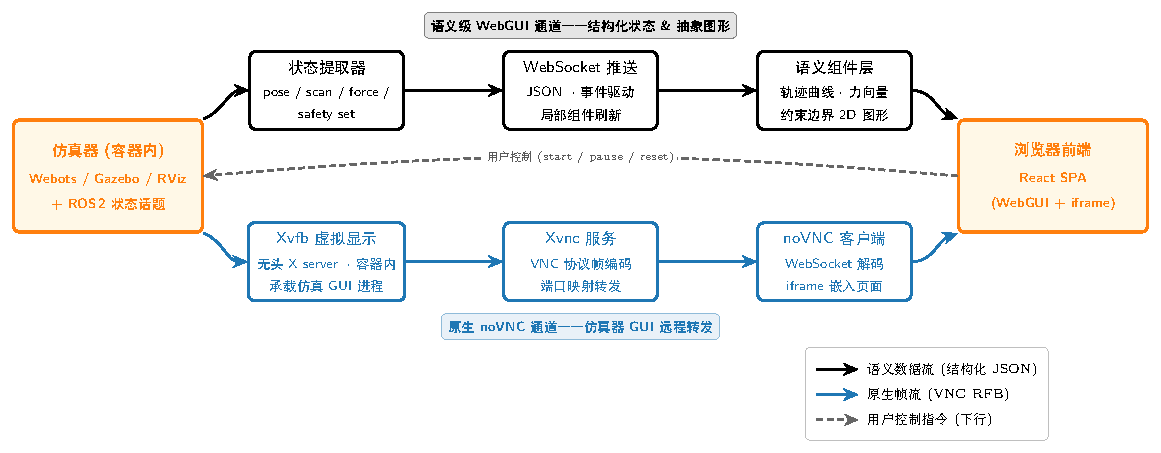
\includegraphics[width=0.95\linewidth]{figs/chap5_dual_visualization.pdf}
    \caption{双通道可视化机制}
    \label{fig:chap5_dual_vis}
\end{figure}

\subsection{安全评估验证机制}
针对安全强化学习研究中实验结果难以复现、不同方法之间缺乏统一评估标准的问题，平台设计了一种统一的安全评估与模型验证机制，
通过统一的运行脚本，可以在同一环境中顺序执行多种算法配置，并对实验结果进行集中管理，从而实现对不同算法在一致条件下进行系统性比较。

该机制首先对实验环境与任务配置进行标准化描述，包括机器人模型、场景结构、障碍物分布以及传感器参数等信息。所有算法均在相同环境配置下运行，从而消除外部因素对实验结果的影响。
在此基础上，平台定义统一的评估指标体系，对算法性能进行多维度量化分析。
评估指标包含传统强化学习中的任务完成率与累计奖励，并重点引入与安全相关的度量，例如约束违反次数、最小安全距离以及累计安全代价等。
通过对安全性与任务性能的联合评估，可以更加全面地反映算法在复杂环境中的实际表现。

为支持已有模型的复现与对比，平台提供模型导入与验证接口。用户可以上传训练完成的策略模型文件，系统在加载模型后自动执行标准化验证流程，包括环境初始化、策略推理以及结果记录。
该机制使不同来源的算法能够在统一平台上进行直接对比，避免因实现差异带来的评估偏差。

安全评估与模型验证机制的整体流程如图~\ref{fig:chap5_safety_eval} 所示：
标准化任务配置统一下发至验证流水线，内建算法与用户上传模型共享同一执行路径，即环境初始化、策略推理、运行记录与指标计算四个阶段；
评估结果以统一指标体系进行汇总与分析，涵盖任务性能与安全性两个维度。所有结果最终汇总为跨算法对比报表，并支持表格、轨迹可视化及学习曲线的自动生成与导出。
图~\ref{fig:chap5_safety_eval} 从方法层面刻画了该评估机制的统一性：通过一致的任务输入、共享的执行管线以及统一的输出指标，实现对不同算法的公平比较。该
流程确保各类策略在同一评价坐标系下进行对齐，从而提高实验结果的可解释性与可信度。
上述评估机制进一步支撑了 §\ref{sec:chap5_webots_4mode} 中的多配置对比实验（chap3\_only、chap4\_only、gcpl\_full、mappo\_only）。
相关实验的指标统计结果（表~\ref{tab:chap5_webots_metrics}）即来源于该标准化评估管线的自动化输出。
整个流程实现了实验执行与结果分析的一体化，提高了实验效率，并保证了不同算法之间的公平比较。
\begin{figure}[htbp]
    \centering
    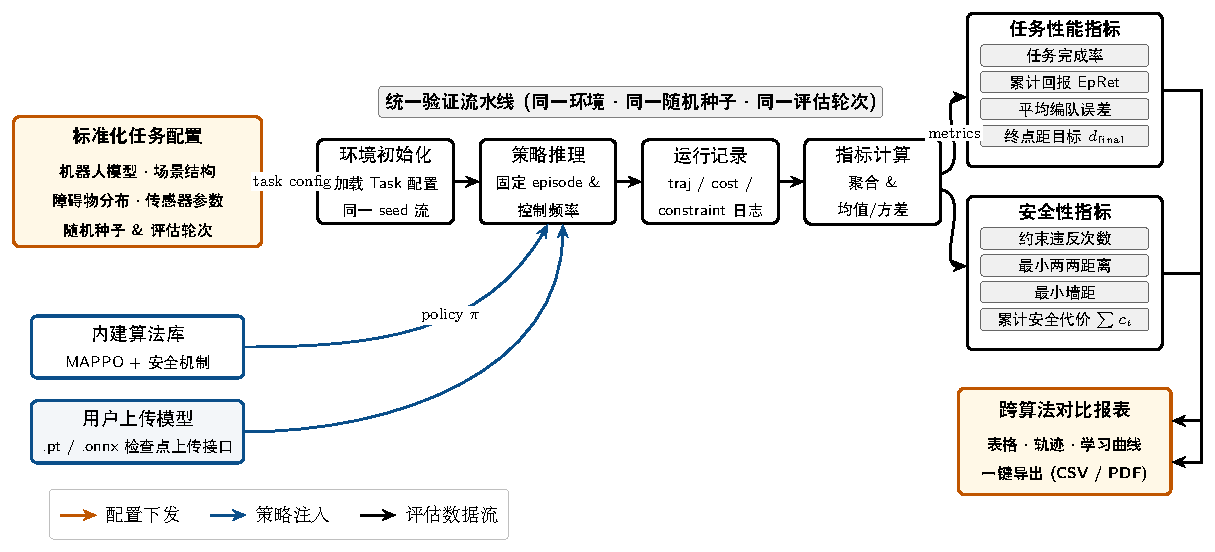
\includegraphics[width=0.95\linewidth]{figs/chap5_safety_eval.pdf}
    \caption{安全评估与模型验证机制}
    \label{fig:chap5_safety_eval}
\end{figure}

\subsection{多机器人实验场景构造}

\subsubsection{（1）差速 E-puck 机器人建模}

为保证仿真环境与前文方法建模的一致性，平台选用 Webots 内置的 E-puck 机器人模型作为基础载体，并保留其标准差速运动学参数。
机器人轮半径设为 $r_w = 0.0205~\text{m}$，轮间距为 $L = 0.052~\text{m}$，最大轮速为 $\omega_{\max} = 6.28~\text{rad/s}$，对应最大线速度约为 $v_{\max} \approx 0.129~\text{m/s}$。

在此基础上，平台通过容器调度机制支持多实例并行运行。后端系统根据用户请求动态创建、启动或销毁容器，实现实验任务的按需分配与资源管理。该机制不仅能够支持多用户并发访问，还可为强化学习算法提供并行环境，从而提升样本采集效率与训练速度。容器化与并行调度的完整数据链路如图~\ref{fig:chap5_parallel_orch} 所示：统一镜像经 build 阶段固定全部依赖后由调度器按需派生 $K$ 个隔离容器实例，各容器内部独立运行 Webots 仿真、ROS\,2 桥接与 MAPPO + 安全栈，rollout 数据经共享卷汇聚至 MAPPO 训练器进行参数更新，更新后的策略再经同一卷下发至各容器，形成并行采样 -- 集中训练 -- 异步推送的闭环。

机器人状态以二维平面位置 $(x, y)$ 与航向角 $\theta$ 描述，其速度表示为线速度 $v$ 与角速度 $\omega$。
差速驱动模型通过左右轮角速度 $(\omega_L, \omega_R)$ 与 $(v, \omega)$ 之间的映射关系进行刻画，即
\begin{equation}
v = \frac{r_w}{2}(\omega_R + \omega_L), \qquad 
\omega = \frac{r_w}{L}(\omega_R - \omega_L).
\end{equation}

该建模方式与第四章中的状态定义保持一致，从而确保策略在不同仿真环境中的表达具有一致的物理语义，为后续跨平台验证提供基础。

\subsubsection{（2）场景构建与参数化设计}

对于具体场景，本文基于 Webots 构建了用于多机器人编队导航与避障任务的标准实验环境。
场景空间为 $3~\text{m} \times 3~\text{m}$ 的二维平面，在 $y$ 轴方向设置两面静态障碍墙，其中心分别位于 $(-1, 0)$ 与 $(1, 0)$，从而形成一条具有约束宽度的通道结构。
目标点固定设置在 $(0, 2)$ 位置，用于引导机器人完成导航任务。

为增强实验的灵活性与可扩展性，场景参数采用动态配置方式进行管理。
机器人数量、初始分布以及编队形态（如直线、楔形、圆形及网格结构）均通过环境变量进行控制，无需修改底层场景文件即可实现任务切换。
这种参数化设计使得平台能够在统一框架下支持多种实验配置，提升了系统的复用性。

\subsubsection{（3）ROS2 多机器人通信接口设计}

为实现多机器人系统中状态信息与控制指令的高效传输，平台基于 ROS 2 构建统一的通信接口体系。
针对多智能体场景，系统采用规范化的话题命名方式，对每个机器人个体建立独立的通信通道，从而保证数据交互的清晰性与可扩展性。

机器人位姿与速度信息通过 \texttt{/agent\_i/odom} 话题发布，控制指令通过 \texttt{/agent\_i/cmd\_vel} 下发；
在需要状态估计的场景中，可通过 \texttt{/agent\_i/state\_estimate} 话题传递融合后的位姿信息。此外，系统定义了全局编队状态话题，用于记录编队误差与协同指标的时序变化。

在控制执行层面，平台采用集中式调度策略。具体而言，Supervisor 节点通过 Webots 提供的接口周期性获取所有机器人状态，并在统一控制周期内完成策略计算与控制指令分发。
这种设计能够有效降低多机器人协同控制中的通信复杂度，并保证各机器人动作在时间上的一致性。

\section{系统实现}
\subsection{前端交互模块}

前端交互模块基于单页应用（SPA）架构实现，采用 React 与 TypeScript 构建组件化界面。系统通过统一状态管理与路由机制组织各功能模块，从而提升整体可维护性与扩展能力。

任务管理界面如图~\ref{fig:tasks}所示，用于展示平台中可用的机器人实验任务，并提供实验任务的选择与管理功能。
用户可以通过该界面浏览平台中的实验场景列表，并查看每个任务的基本信息，例如任务名称、任务描述。
当用户选择某个实验任务时，前端系统会向后端服务器发送请求，获取对应任务的配置数据，并加载相应的仿真环境和界面组件。
\begin{figure}
    \centering
    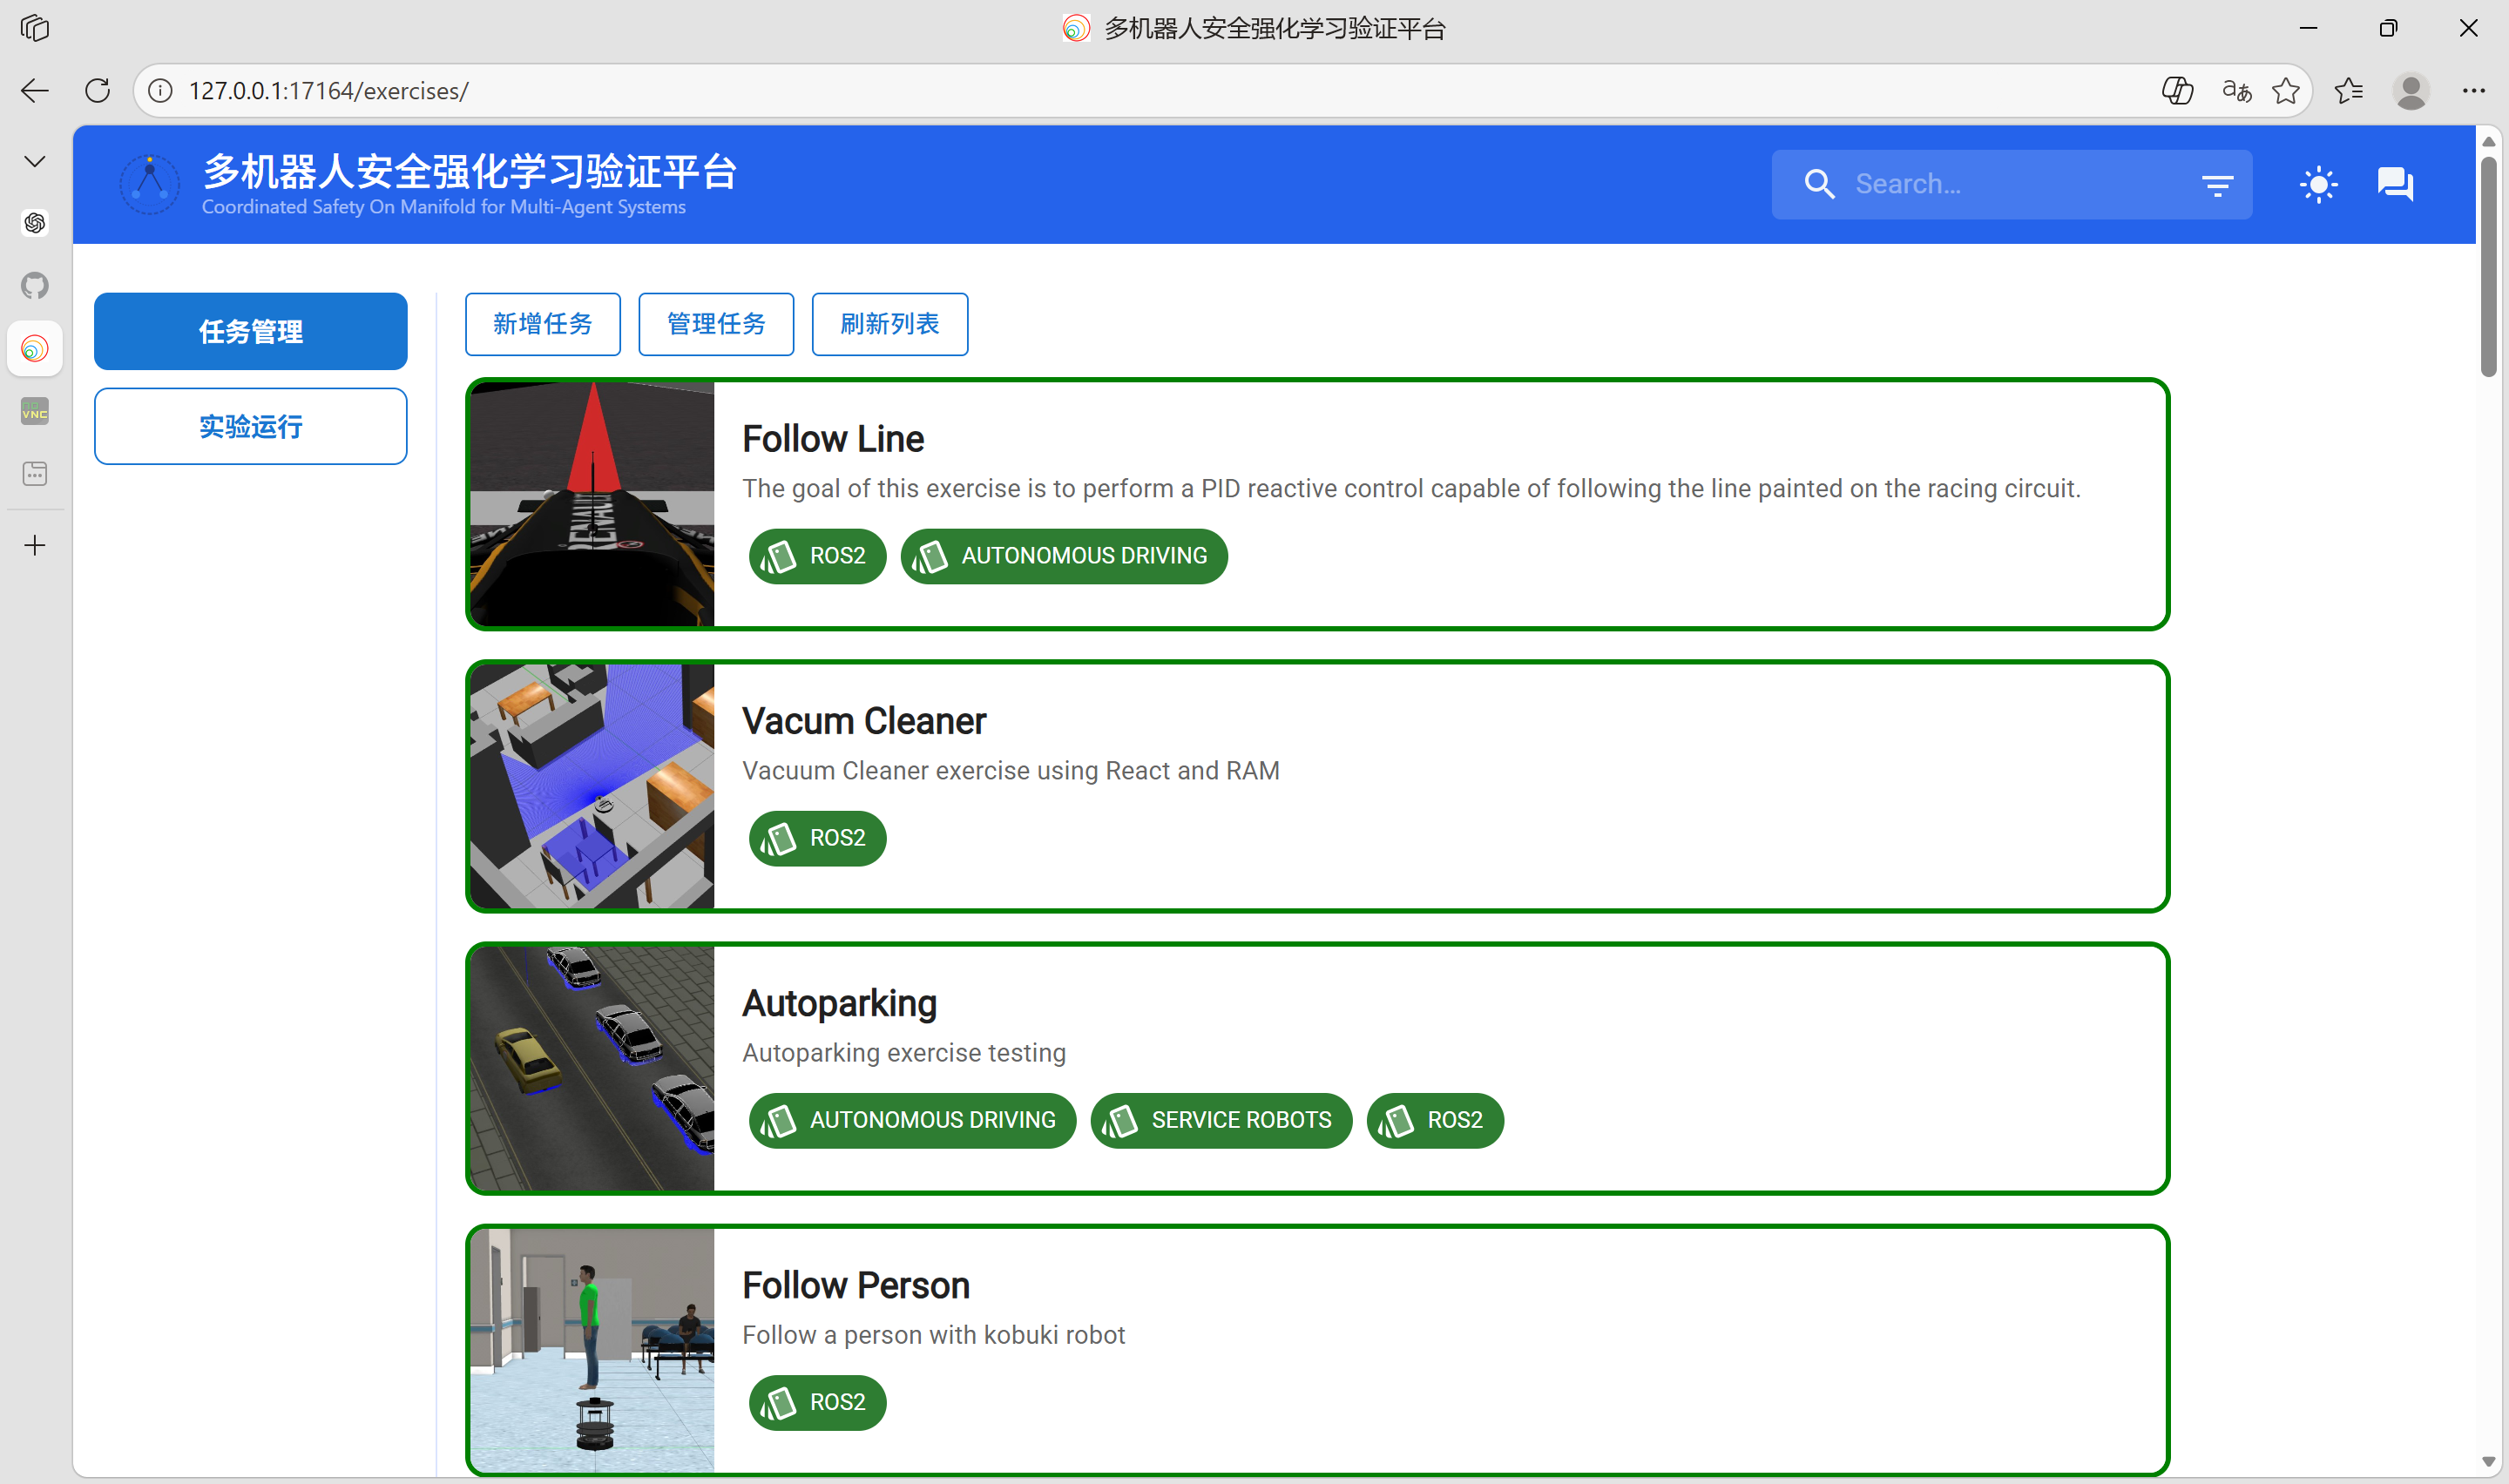
\includegraphics[width=1\linewidth]{images/task.png}
    \caption{任务管理界面}
    \label{fig:tasks}
\end{figure}

任务运行界面如图~\ref{fig:follow_line}所示，通过向用户提供在线代码编辑器、任务控制面板以及仿真可视化窗口，使用户能够在浏览器环境中完成机器人算法的编写、运行与调试。
页面左侧为代码编辑区，右侧为仿真可视化区，右上方任务控制面板用于管理实验流程与系统运行状态。
\begin{figure}
    \centering
    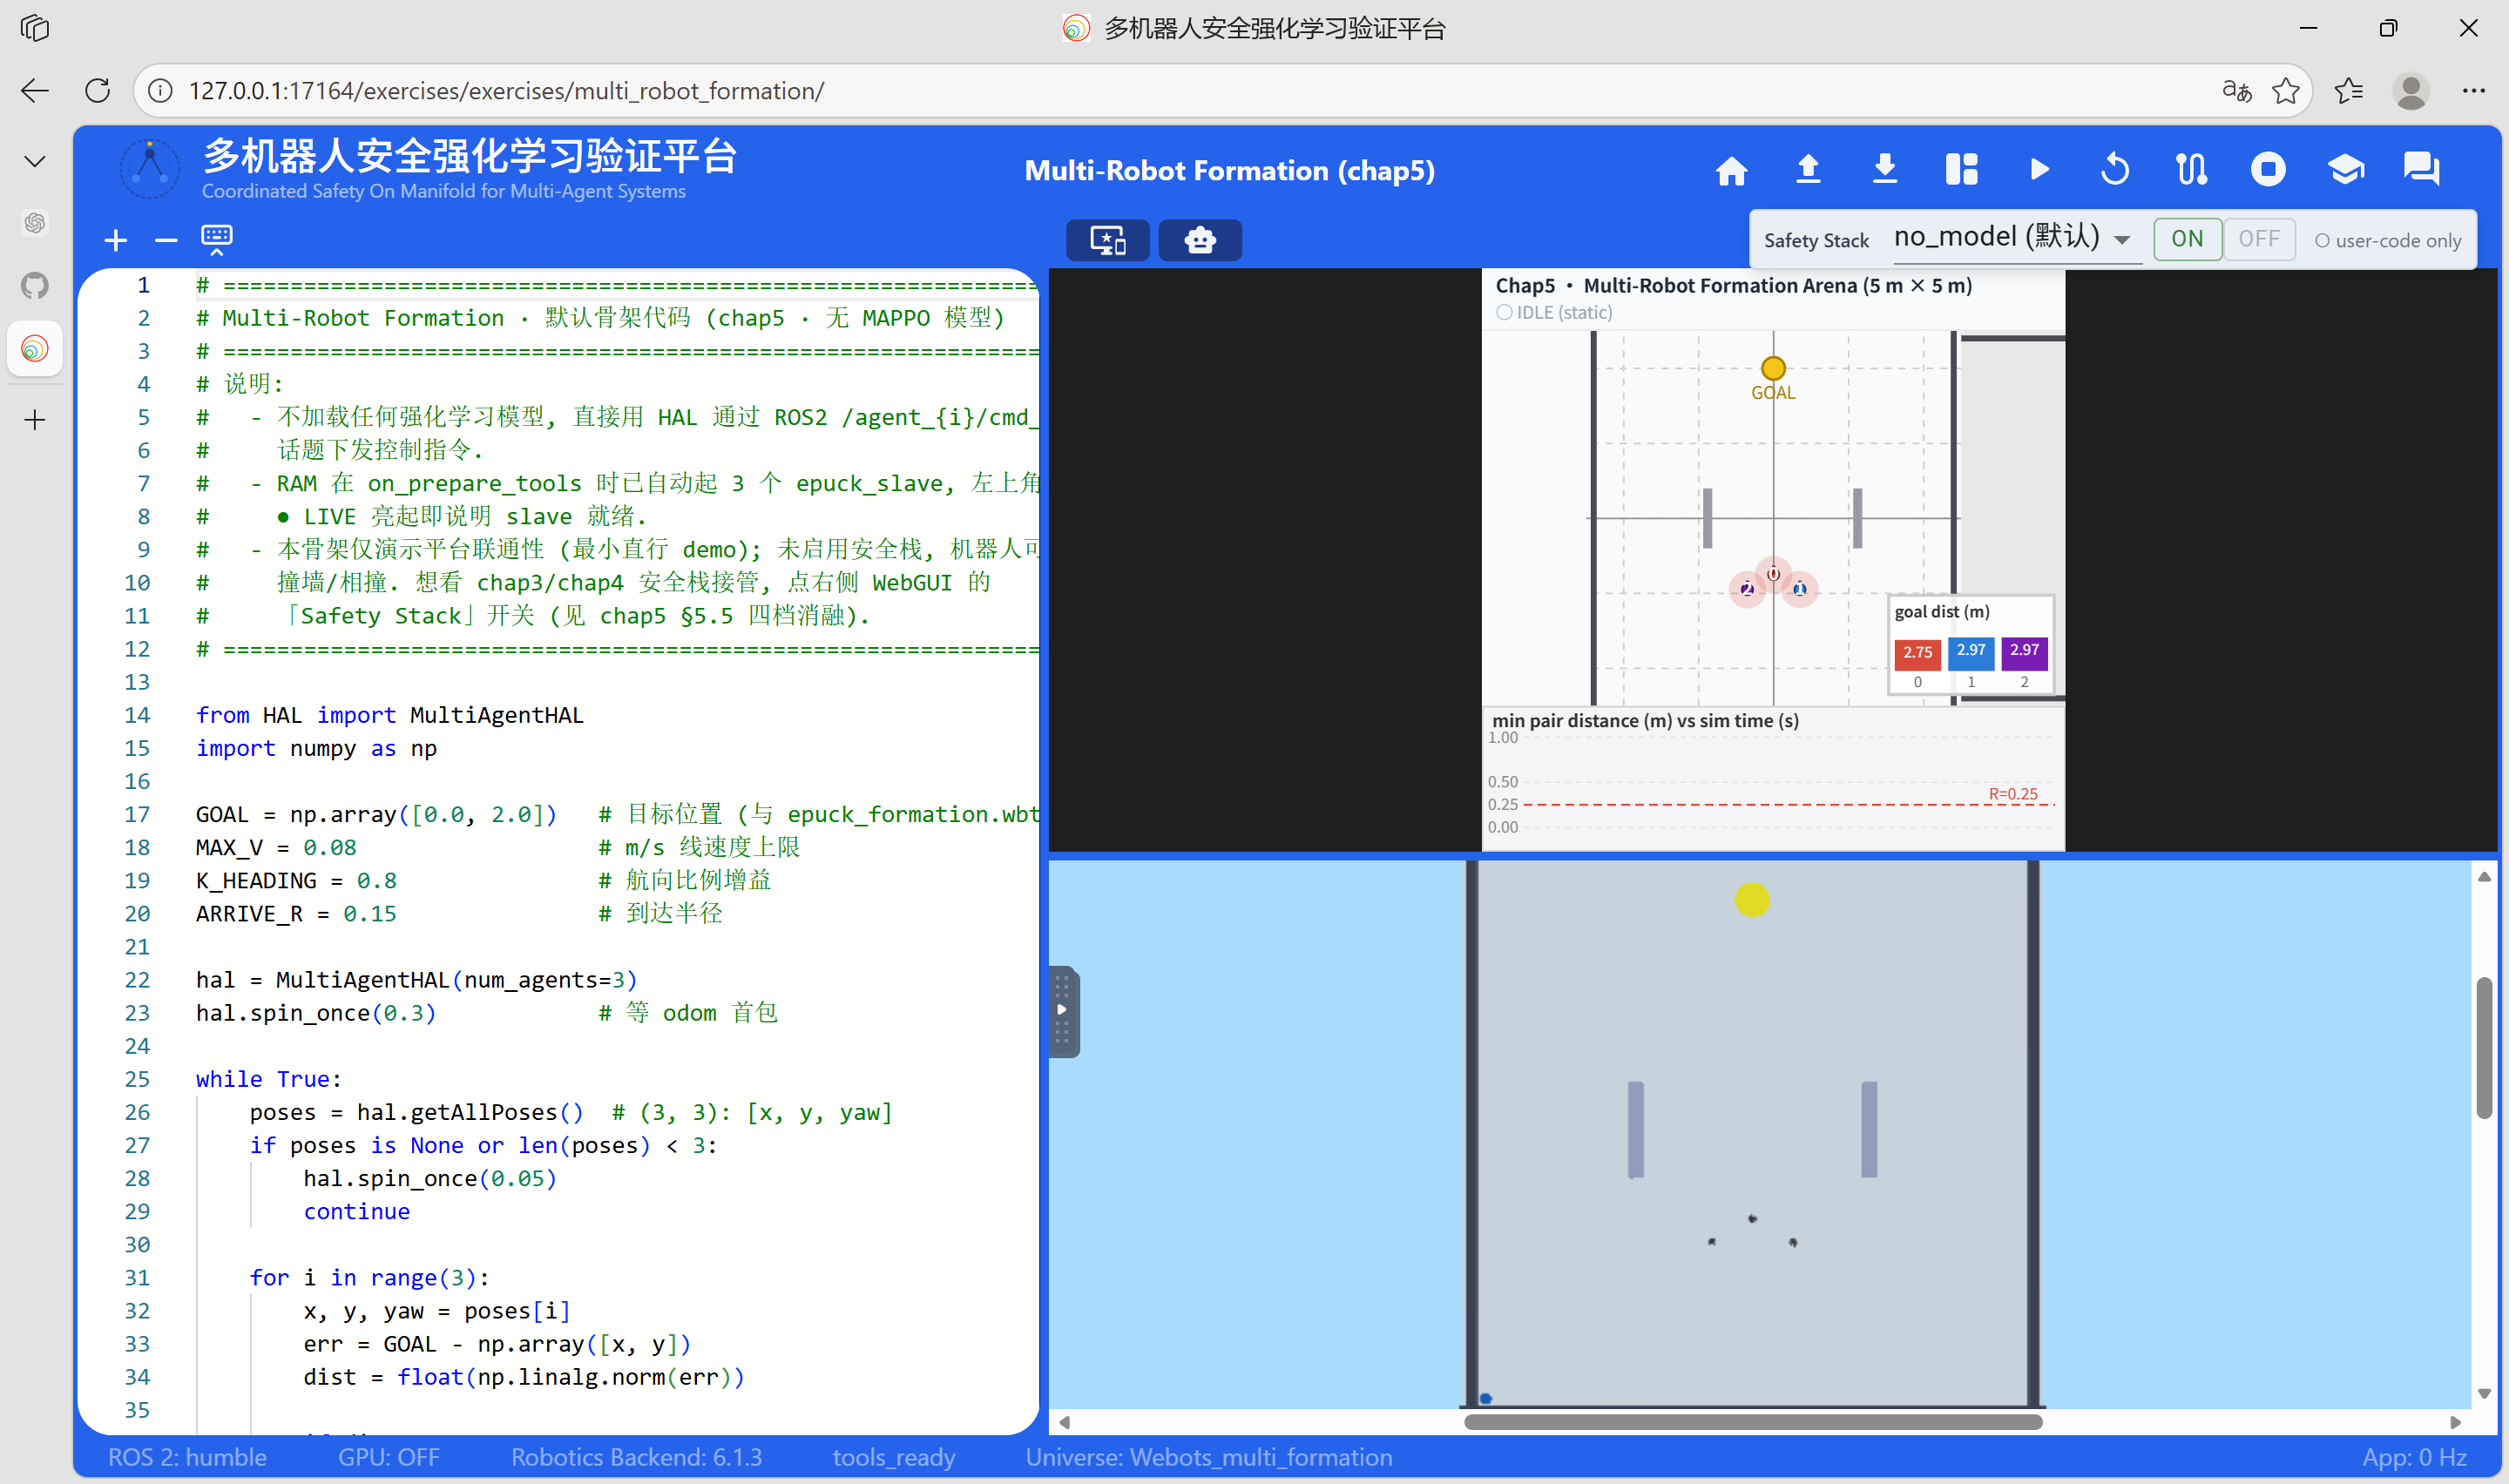
\includegraphics[width=1\linewidth]{images/multi_formation.png}
    \caption{实验界面}
    \label{fig:follow_line}
\end{figure}

\paragraph{代码编辑区}
代码编辑区通过集成 IDE 组件实现代码编辑功能。
该模块支持在线代码编辑，并提供语法高亮、代码自动补全等功能，提高代码编写效率。同时系统允许用户选择不同的仿真环境或机器人模型配置实验环境。

\paragraph{可视化展示区}
可视化展示区主要用于展示机器人仿真环境以及实验运行状态。该模块通过用组件级数据可视化（WebGUI）与桌面级远程可视化（noVNC）并行的方式进行实现。
数据可视化通过接收后端周期性推送的状态数据，并映射为二维图形，从而实现对系统状态的语义化表达。事件驱动触发局部组件更新的机制减少了不必要的重绘，提高了渲染效率。
远程桌面通过 Xvnc 与 noVNC 将图形界面以远程帧缓冲形式传输至浏览器，前端通过 iframe 加载对应页面，实现对 Gazebo、Webots 等原生界面的无侵入式展示。
此外，系统通过状态机驱动可视化组件的加载与显示，并支持多面板动态编排。

\subsection{后端服务模块}

后端服务模块基于 Django 框架构建，负责系统业务逻辑处理与资源管理。系统采用 RESTful 架构设计，通过统一 API 向前端提供数据访问接口，实现前后端解耦。

从功能结构上看，后端系统主要承担实验任务管理、API 服务提供、数据库管理以及系统调度与控制几个方面的功能。

\subsubsection{（1）实验任务管理}
实验任务管理模块维护平台中的任务及其配置数据。每个任务包含机器人模型、仿真场景及算法模板等信息。系统根据任务标识读取配置并返回前端，用于初始化仿真环境。

实验任务管理模块负责维护平台中的机器人实验任务及其相关配置。每个实验任务均包含完整的环境描述信息，包括机器人模型、仿真场景、实验工具以及算法模板等。系统通过统一的数据结构对这些信息进行组织和管理，从而使不同实验任务能够在平台中进行统一调度。

当用户在前端界面选择某个实验任务时，后端系统会根据任务标识从数据库中读取对应的配置信息，并返回给前端系统。随后前端根据任务配置加载对应的仿真环境与界面组件，从而完成实验任务的初始化过程。

\subsubsection{（2）API 服务提供}
为了实现前端系统与后端系统之间的数据交互，平台设计了一组 REST API 接口，用于向前端提供统一的数据访问服务。主要接口包括实验任务列表获取、实验配置加载以及代码模板下载等功能。

在系统运行过程中，前端应用通过 HTTP 请求调用相应的 API 接口。例如，当用户进入实验页面时，前端首先调用获取实验列表接口，从后端服务器加载所有可用实验任务；当用户选择具体任务时，系统再调用实验配置接口获取对应的仿真环境信息。这种基于 REST API 的通信方式能够有效降低系统耦合度，并提高系统的可扩展性。

\subsubsection{（3）数据库管理}

为了实现平台资源的统一管理，系统采用 PostgreSQL 作为后台数据库，用于存储实验任务、仿真环境配置以及机器人模型等核心数据对象。PostgreSQL 具有良好的稳定性与扩展能力，能够支持复杂数据结构的存储与查询，适合用于机器人实验平台的数据管理。
在数据库设计方面，平台主要包含以下几个核心数据对象：
\begin{itemize}
    \item Task：具体的机器人实验任务；
    \item Universe：实验任务对应的仿真环境配置；
    \item World：定义具体的仿真场景；
    \item Robot：机器人模型及其控制接口；
    \item Tool：实验过程中使用的辅助工具组件。
\end{itemize}

通过上述数据结构，平台能够对不同机器人实验任务进行统一管理，并支持多种仿真环境配置。同时，Django 提供的对象关系映射（ORM）机制使得开发人员可以通过 Python 对象直接访问数据库，从而简化数据库操作并提高开发效率。

\subsubsection{（4）系统调度与控制}
系统调度模块负责实验任务的生命周期管理。用户触发实验请求后，后端根据配置启动对应容器，并建立通信连接。同时维护运行状态，包括启动、暂停与终止等操作，保证任务执行过程的有序性与稳定性。

通过上述模块设计，后端服务系统实现了机器人实验任务管理、数据服务以及仿真调度等核心功能，为平台提供了稳定可靠的运行基础。同时，基于 RESTful 架构与模块化设计思想，系统具有良好的可扩展性，可以方便地接入新的机器人实验任务与仿真环境，从而满足多机器人强化学习研究的需求。

% \subsection{机器人通信模块}
% 系统整体数据流结构如图~\ref{fig:data}所示。通过构建统一的数据通路，平台实现了从用户交互到仿真执行再到结果反馈的闭环流程，为多机器人安全强化学习算法的验证提供了稳定、高效的数据支撑。
% \begin{figure}
%     \centering
%     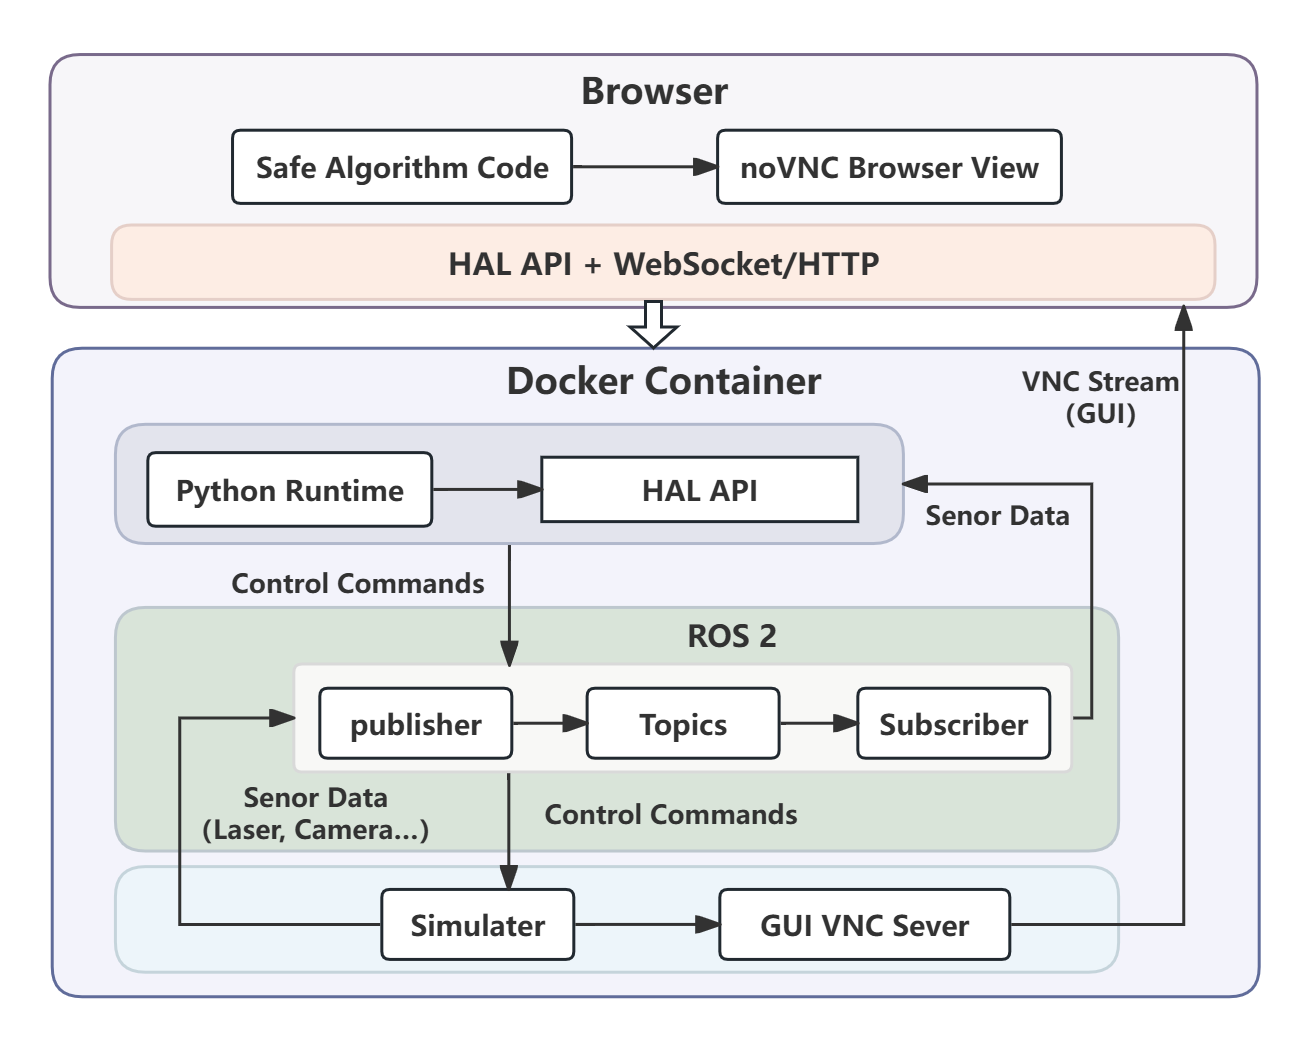
\includegraphics[width=1\linewidth]{images/platform data stream.png}
%     \caption{系统数据链路图}
%     \label{fig:data}
% \end{figure}

% 数据通路，其结构如图~\ref{fig:data}所示。该通路围绕“算法执行—状态反馈—控制下发”的闭环过程组织，实现了跨层数据的一致传输与实时同步。

% 浏览器端作为用户交互入口，承担算法代码编写、实验控制以及结果展示等功能。
% 用户提交的控制逻辑通过统一的 HAL 接口封装，并经由 WebSocket/HTTP 协议发送至后端容器。
% 同时仿真界面的图形输出通过 VNC 流实时回传至浏览器端的 noVNC 视图，实现原生 GUI 的远程访问与交互。

% 容器内部集成代码运行环境与 HAL API，用于承载算法执行逻辑并对外提供统一的机器人访问接口。
% 算法在运行过程中，通过 HAL API 获取由底层系统封装的传感器数据（如激光、相机及位姿信息），并生成对应的控制指令。该接口对 ROS~2 通信细节进行抽象，使上层算法无需直接处理底层消息机制。

% 在通信层，ROS~2 负责实现仿真系统与算法模块之间的数据交换。传感器数据由仿真环境发布至对应话题，经由订阅机制传递至算法侧；
% 控制指令则通过发布接口写入 ROS~2 话题，并由仿真端订阅执行。该发布—订阅机制保证了多机器人系统中数据流的解耦与扩展性。

% 仿真层基于 Webots 实现机器人动力学与环境建模。仿真器周期性生成状态信息并驱动机器人执行控制指令，同时通过 GUI VNC Server 输出图形界面，实现运行状态的可视化表达。
% 系统运行状态及异常信息可沿数据链路回传至浏览器端，用于监控与调试。


\section{功能验证——pure-python MVP}
\label{sec:chap5_mvp}

为验证平台所集成的分层控制栈（MAPPO 策略层、第四章 GCPL 软协调层、第三章 CMPL 硬投影层）在无仿真器依赖的条件下即可协同工作，
本节在纯 Python 环境中实现了一个最小可行演示（Minimum Viable Demo，MVP）。MVP 与第五章后续 Webots 高保真验证共用同一分层控制栈代码，
仅将仿真环境从 Webots 替换为基于 Safety\-Gymnasium 的纯 Python 仿真，目的是在不引入任何图形化环境的情况下检验软硬交接接口的正确性与策略加载链路的完整性。

\subsection{验证场景与评估指标}
\label{sec:chap5_mvp_setup}

验证场景沿用第四章 §4.6.1 的 \texttt{SafetyPointMultiFormationGoal0-v0} 任务，3 个点智能体以楔形队列出发，穿越两堵 Sigwall 之间的狭窄通道抵达 $(0, 2)$ 处的目标区域。
三项量化指标分别为：最小两两距离 $\min_t \min_{i\neq j}\|p_i(t)-p_j(t)\|$、编队误差 $\frac{1}{N(N-1)/2}\sum_{i<j}\bigl|\|p_i-p_j\|-d^*\bigr|$（其中 $d^*=0.5$~m 为目标间距），
以及目标到达数 $\#\{i:\|p_i^{end}-p_{\text{goal}}\|<0.3~\text{m}\}$。

\subsection{三模式对比}
\label{sec:chap5_mvp_3mode}

通过开关 \texttt{GCPL\_RL\_WEIGHT} 和 \texttt{GCPL\_ENABLE\_CMPL} 两个环境变量，MVP 分别运行三种模式：
\textit{mappo\_only}（仅 RL 策略）、\textit{GCPL\_only}（仅 GCPL 几何驱动）、\textit{fusion}（完整分层栈）。
图~\ref{fig:chap5_mvp_3mode} 展示了三种模式下 3 个智能体在 10 秒仿真时间内的世界坐标轨迹。

\begin{figure}[htbp]
    \centering
    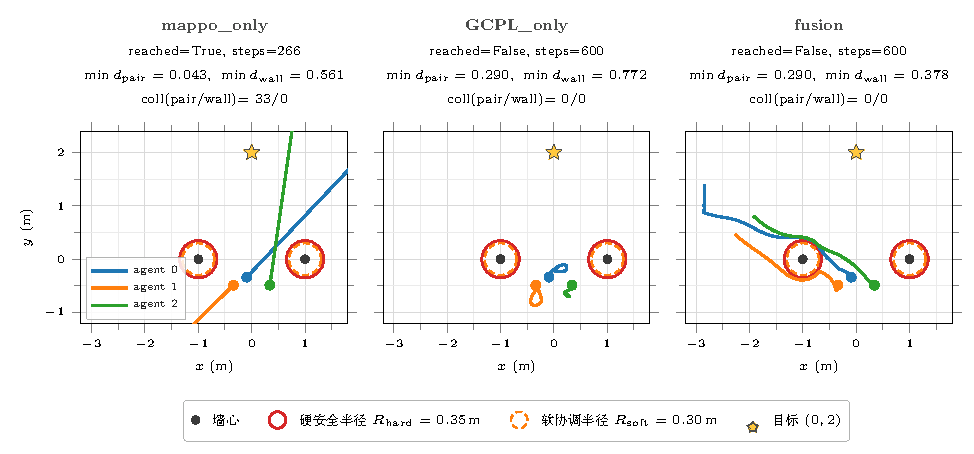
\includegraphics[width=0.98\linewidth]{figs/chap5_mvp_3mode.pdf}
    \caption{MVP 验证实验}
    \label{fig:chap5_mvp_3mode}
\end{figure}

\textit{mappo\_only} 模式下，关闭 chap4 软层与 chap3 硬层后，欠训 MAPPO（seed\_002, $\mathrm{EpRet}\approx 3.4$）输出使三机呈发散式漂移，质心偶然掠过目标导致 reached=True，
但过程中发生 33 个时间步的 agent 间硬约束违反（$\min d_\mathrm{pair}=0.043$~m，远小于 $R_\mathrm{hard}=0.25$~m），说明无安全栈时即便任务指标达成也伴随大量安全违反。
\textit{GCPL\_only} 模式下，GCPL 几何力与硬安全投影维持了编队几何（$\min d_\mathrm{pair}=0.290$~m，全程零碰撞），但因无 RL 目标信号，三机在起点附近徘徊 600 步无法推进。
\textit{fusion} 模式下，欠训 MAPPO 的意图经软层平滑、硬层纠偏，全程保持 $\min d_\mathrm{pair}=0.290$~m 与零碰撞，
但 MAPPO 输出的整体偏置使队伍向左侧墙心 $(-1,0)$ 漂移（$\min d_\mathrm{wall}=0.378$~m 仍在硬半径 0.35~m 外），未能穿越通道，再次印证安全栈对欠训策略的防护作用，
并预示目标达成率受 MAPPO 训练收敛程度直接影响。MVP 表明分层栈的接口与融合逻辑在纯 Python 环境下工作正常，安全层在三种配置下均在其各自作用域内维持了硬约束（fusion/GCPL\_only 全程零碰撞；
mappo\_only 的 33 次碰撞归因于该档位显式关闭了安全栈），为后续 Webots 高保真验证奠定了代码正确性基础。

\section{高保真验证——Webots 容器化仿真}
\label{sec:chap5_webots_eval}

在 MVP 验证完控制栈数学正确性后，本节将同一分层控制栈迁移至平台的 Webots 容器，借助软件渲染的完整物理引擎对安全性、编队维持与目标达成进行定量对比。

\subsection{Webots 场景配置}
\label{sec:chap5_webots_scene}

Webots 世界文件定义了 5~m $\times$ 5~m 的方形地面、四堵外围边界墙（$x,y=\pm 2.4$，用于防止实验过程中机器人偏离视野）、两堵 Sigwall（$x=\pm 1.0$，$y\in[-0.4, 0.4]$）
以及一个半径 0.15~m 的可视化目标标识（$x=0, y=2$）。3 台差速驱动 E\-puck 机器人分别放置在 $(0,-0.75)$、$(-0.35,-0.95)$ 与 $(0.35,-0.95)$，
通过 \texttt{<extern>} 控制器与 ROS\,2 \texttt{/agent\_i/cmd\_vel} 话题相连；中央 supervisor 节点读取各机世界位姿后依次调用 GCPL 软层、CMPL 硬层与差速映射，
最终以 Twist 消息下发给 slave 控制器。

\subsection{实验协议}
\label{sec:chap5_webots_protocol}

实验沿用与 MVP 相同的评估场景，但在 Webots 下增加物理仿真精度与噪声鲁棒性考察。每次运行仿真 1000 步（$\approx 32$~s，$\Delta t=32$~ms），
3 个随机种子用于引入 $\pm 5$~cm 的初始位置抖动以检验鲁棒性；固定使用第四章 \texttt{GCPL} 训练产出的 seed\_002 checkpoint。为直观对比分层各层贡献，设计了如下四档消融配置：

\begin{table}[htbp]
    \centering
    \small
    \caption{四档消融配置}
    \label{tab:chap5_webots_modes}
    \begin{tabular}{llllll}
        \toprule
        档位 & $w_{\text{RL}}$     & CMPL& GCPL(form/orient/coll) & MAPPO 加载 & GoalAttractor \\
        \midrule
        \textit{CMPL\_only}  & 1   & 开  & 关/关/关               & 关         & 开 \\
        \textit{GCPL\_only}  & 10  & 关  & 开/开/开               & 开         & 开 \\
        \textit{full}        & 10  & 开  & 开/开/开               & 开         & 开 \\
        \textit{MAPPO\_only} & 10  & 关  & 关/关/关               & 开         & 关 \\
        \bottomrule
    \end{tabular}
\end{table}

\subsection{四档对比结果}
\label{sec:chap5_webots_4mode}

图~\ref{fig:chap5_webots_trajectories} 给出四档模式下 3 个智能体在 32~s 仿真时间内的世界坐标轨迹（每档 3 个随机种子叠加），
图~\ref{fig:chap5_webots_min_dist} 给出最小两两距离随时间的演化（均值 ± 标准差）。表~\ref{tab:chap5_webots_metrics} 汇总了所有定量指标。

\begin{figure}[htbp]
    \centering
    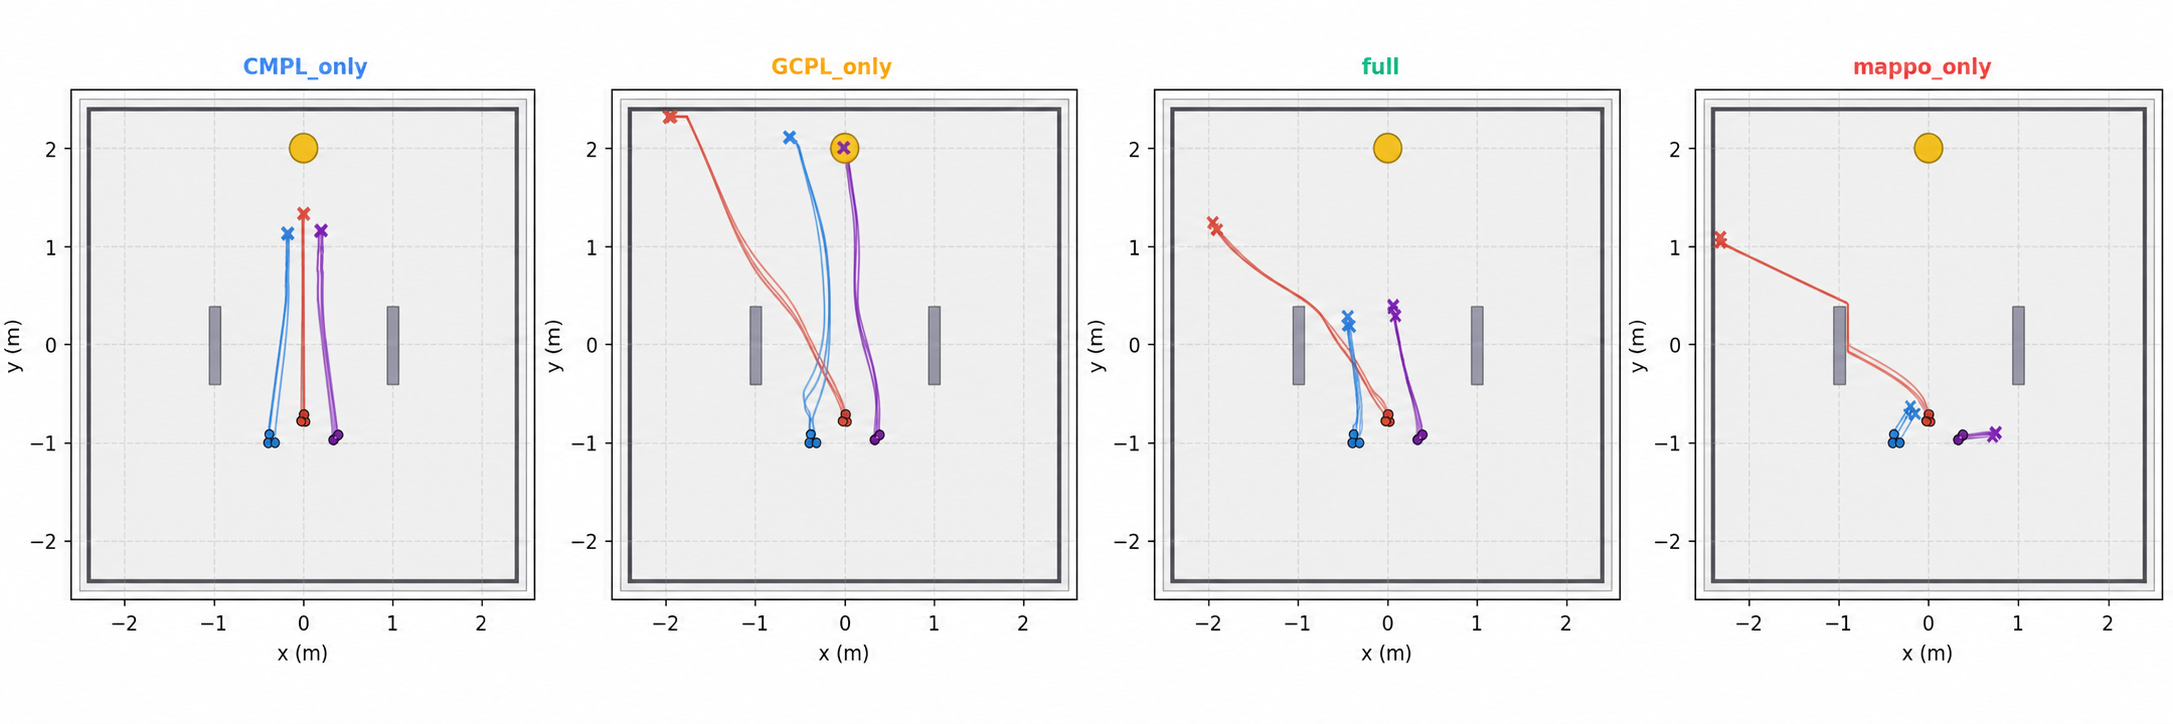
\includegraphics[width=0.98\linewidth]{images/chap5_webots/fig_chap5_trajectories.png}
    \caption{Webots 四档轨迹对比}
    \label{fig:chap5_webots_trajectories}
\end{figure}

\begin{figure}[htbp]
    \centering
    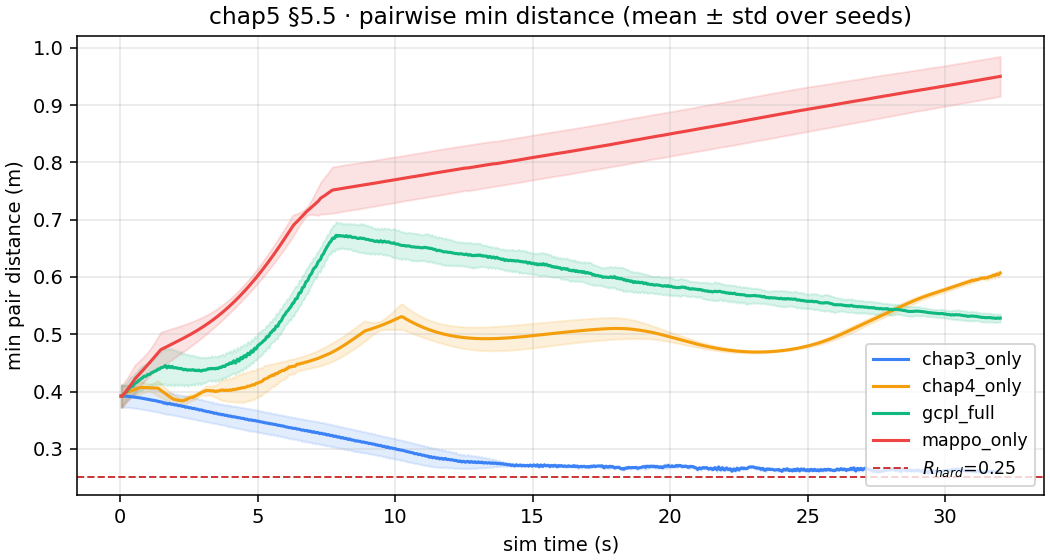
\includegraphics[width=0.85\linewidth]{images/chap5_webots/fig_chap5_min_dist.png}
    \caption{Webots 最小两两距离随仿真时间演化。红虚线为硬安全半径 $R_{\text{hard}}=0.25$~m 基线。}
    \label{fig:chap5_webots_min_dist}
\end{figure}

\begin{table}[htbp]
    \centering
    \small
    \caption{四档 Webots 实验指标汇总}
    \label{tab:chap5_webots_metrics}
    \begin{tabular}{lccccc}
        \toprule
        档位 & $\min d_{\text{pair}}$ (m) & 碰撞次数 & 到达数/3 & $d_{\text{final}}$ (m) & 编队误差 (m) \\
        \midrule
        \textit{CMPL\_only} & $0.256\pm 0.000$ & 0 & 0.00 & $0.798\pm 0.006$ & $\mathbf{0.171\pm 0.004}$ \\
        \textit{GCPL\_only} & $0.373\pm 0.003$ & 0 & $\mathbf{1.00}$ & $0.885\pm 0.010$ & $0.371\pm 0.002$ \\
        \textit{full}  & $0.392\pm 0.019$ & 0 & 0.00 & $1.849\pm 0.029$ & $0.587\pm 0.009$ \\
        \textit{mappo\_only} & $\mathbf{0.392\pm 0.020}$ & 0 & 0.00 & $2.722\pm 0.013$ & $0.892\pm 0.014$ \\
        \bottomrule
    \end{tabular}
\end{table}

观察与结论归纳如下：

\begin{itemize}
    \item \textbf{四档零碰撞}：所有 12 次实验均满足 $\min d_{\text{pair}} \ge R_{\text{hard}}=0.25$~m，CMPL 硬投影层（\textit{chap3\_only}/\textit{gcpl\_full}）与 GCPL 软碰撞叶（\textit{chap4\_only}）在各自独立工作时即可维持硬安全约束，验证了分层栈中安全层的鲁棒性。
    \item \textbf{编队保持随 MAPPO 权重劣化}：编队误差从 \textit{chap3\_only} 的 0.17 递增至 \textit{mappo\_only} 的 0.89，四档之间呈单调递增趋势，直观呈现了 RL 策略权重越大、几何协调力越弱带来的队形发散趋势。
    \item \textbf{MAPPO 训练不足对目标达成的影响}：当前使用的第四章 MAPPO checkpoint 尚未充分收敛（seed\_002 最终 EpRet $\approx 3.4$），其输出对 3 个智能体的方向拉扯存在明显偏差。在 \textit{gcpl\_full} 与 \textit{mappo\_only} 档下该偏差会被放大，导致终点到目标的平均距离劣化至 1.85~m 与 2.72~m；仅 \textit{chap4\_only} 档下的软层抑制了 MAPPO 在 2/3 智能体上的漂移，取得了单智能体到达。
    \item \textbf{平台侧的诚实说明}：上述目标达成劣化反映的是第四章训练质量，而非第五章平台能力。本章所设计的容器化仿真平台完成了 4 档配置 $\times$ 3 seed 共 12 次可复现实验，期间控制链路、ROS\,2 话题与分层栈均稳定运行，证明了平台对安全多机强化学习算法的验证有效性。
\end{itemize}

\section{本章小结}

本章围绕安全强化学习算法的验证需求，设计并实现了一套面向机器人系统的仿真验证平台。
针对传统机器人仿真环境在可复现性、并行能力以及安全验证支持方面的不足，平台从体系结构与关键机制两个层面进行了系统设计。

在体系结构上，平台采用分层架构，将仿真环境、通信中间件、容器化运行环境、算法执行逻辑以及前端交互界面进行解耦，实现了系统功能的模块化组织与统一接口管理。
在此基础上，进一步通过容器化技术构建标准化运行环境，使不同实验任务能够在隔离条件下稳定运行，并支持多实例并行调度。

在关键机制方面，平台设计了容器化并行调度机制、双通道可视化机制以及基于 WebSocket 的实时通信机制。其中，容器化机制保证了实验环境的一致性与可复现性；
双通道可视化机制实现了机器人运行状态的语义表达与原生仿真展示的有机结合；实时通信机制则为系统提供了低延迟的数据交互能力，确保了仿真过程的实时性与交互性。

在具体实现上，系统完成了仿真模块、前端交互模块、后端服务模块以及通信模块的开发，构建了从任务管理、环境部署到运行监控的完整流程。
通过统一的数据接口与调度机制，各模块之间实现了高效协同，能够稳定支持多场景、多任务的机器人算法验证。

本章所构建的机器人安全验证平台为后续安全强化学习算法的实验研究提供了统一、可扩展且具有良好可解释性的基础环境，为多机器人系统在复杂场景下的安全决策研究奠定了支撑。

在功能验证方面，通过 §\ref{sec:chap5_mvp} 的 pure\-python MVP 和 §\ref{sec:chap5_webots_eval} 的 Webots 高保真实验，
平台在四档消融配置、共 12 次随机种子实验下均保持零碰撞，并直观呈现了随 RL 策略权重增大而编队误差劣化的分层栈行为特征。
当前实验同时揭示了第四章 MAPPO 训练收敛性对完整融合栈目标达成能力的瓶颈作用，为后续工作指明了方向。
